\chapter{Casos de Uso}
\label{chapter:casos_de_uso}

% Escrever sobre caso de uso do sistemas
No capítulo \ref{chapter:projeto} descrevemos o funcionamento da Interface e sua comunicação com a linguagem MQTT. Este capítulo busca demonstrar o funcionamento do sistema em hardwares com a interface implementada pelos softwares descritos na seção \ref{section:codigos_fonte} disponível no Apêndice. São aplicações simples que mostram a facilidade e a escalabilidade do sistema, além de demonstrar como o sistema pode ser implementado em plataformas.

\section{Medição de temperaturas de CPU}
\label{section:temp_cpu}

Este exemplo tem como objetivo medir a temperatura da CPU de um console com baseado em suas atividades, serviços e processos em execução. A aplicação pode ser escalada para a obtenção de outras informações da CPU e do sistema, podendo assim disponibilizar análises de desempenho da plataforma, além de montar perfis de uso do sistema e administrar seu uso.

Para isso precisaremos utilizar um Publisher no console a ter informações de temperatura a ser coletadas e um Subscriber para receber estas temperaturas via MQTT e persisti-las em banco de dados. Ambas as aplicações utilizarão as APIs em Javascript, utilizando Node.js para coletar as informações do sistema, implementar o Publisher, o Subscriber, o driver para MongoDB (também disponível em anexo) e a geração de um gráfico utilizando a plataforma plotly \cite{plotly}.


\begin{figure}[h!]
\centering
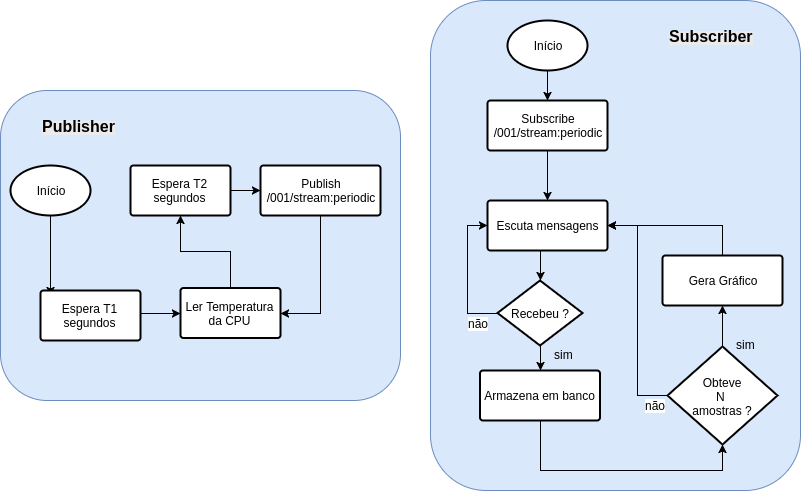
\includegraphics[width=11.5cm]{./02_Capitulos/02_Cap4/figures/fluxo_controle_temp}
\caption{Diagrama de fluxos do Publisher e do Subscriber}
\label{fig:4.1.0/fluxo_controle_temp}
\end{figure}

% Falar sobre o diagrama de fluxo
A \ref{fig:4.1.0/fluxo_controle_temp} mostra todo o fluxo das duas aplicações, o Publisher publica em no tópico \textit{/001/stream:periodic}, a informação coletada a cada T1=3 segundos e espera T2=1 antes de enviar. O Subscriber escuta este tópico e persiste ao chegar uma mensagem de dados pelo Data Stream, ao atingir 100 amostras, um gráfico de Temperatura da CPU principal pela Data-Hora de inserção é gerado com as últimas 100 inserções no banco.


% Inserção no banco


% Visualização com o plotly



